\documentclass{article}

% Language setting
% Replace `english' with e.g. `spanish' to change the document language
\usepackage[russian]{babel}

% Set page size and margins
% Replace `letterpaper' with `a4paper' for UK/EU standard size
\usepackage[a4paper,top=2cm,bottom=2cm,left=3cm,right=3cm,marginparwidth=1.75cm]{geometry}

% Useful packages
\usepackage{amsmath, amssymb, amsthm}
\usepackage{indentfirst}
\usepackage{graphicx, float}
\usepackage[colorlinks=true, allcolors=blue]{hyperref}

\newcommand{\argmin}{\arg\!\min}
\newcommand{\argmax}{\arg\!\max}

\setlength{\parskip}{5pt}
\setlength{\parindent}{20pt}
\title{Эмпирические байесовские нейронные сети}
\author{Басов Дмитрий Константинович}
\date{}
\begin{document}
\maketitle

\begin{abstract}

Данная статья посвящена применению техники эмпирического Байеса к байесовским нейронным сетям. Концептуально идея следующая:
\begin{enumerate}
 \item Мы используем диагональное нормальное распределение для аппроксимации апостериорного распределения весов модели~--- $q(W)$.
 \item Априорное распределение весов модели так же задаётся диагональным распределением с нулевым матожиданием~--- $p(W)$.
 \item Используя вариационный вывод, мы приходим к ситуации, когда ELBO зависит от $KL(q(W) || p(W))$. Так как оба распределения являются нормальными, то KL дивергенция считается аналитически.
 \item Мотивация следующего этапа была взята из RVM~--- взять дисперсию априорного распределения весов модели $p(W)$ из данных. Там несложно берётся производная и всё получается красиво, кроме возможного деления 0/0. Но сделав замену переменных, от этой беды можно уйти.
\end{enumerate}
Пункты 1--3 в принципе были описаны в статье \href{https://arxiv.org/pdf/1505.05424}{Weight Uncertainty in Neural Networks}. А вот четвёртый пункт я ни в книгах, ни в статьях не находил.

\end{abstract}


\section{Обозначения и сокращения}
$N(\mu, \sigma^2)$ --- нормальное распределение

$\mathbf{x} \odot \mathbf{y}$ --- поэлементное произведение (произведение Адамара) векторов

$\mathcal{L}$ --- Evidence Lower Bound (ELBO)

$KL(q || p) = \int_{}{} q(\mathbf{Z}) \cdot \ln{\dfrac{q(\mathbf{Z})}{p(\mathbf{Z})}} d\mathbf{Z}$ --- дивергенция Кульбака --- Лейблера

$\mathbf{x}$ --- вектор признаков

$\mathbf{y}$ --- вектор целевой переменной

$D$ --- датасет --- пары значений \{$\mathbf{x_i}$, $\mathbf{y_i}$\}, где $i = 1, \dots, L$

$\mathbf{W}$ --- веса модели --- случайная величина размерности M

$p(D | \mathbf{W}) = \prod_{i=1}^{L} p(\mathbf{y_i} | \mathbf{x_i}, \mathbf{W})$ — правдоподобие (likelihood)

$p(\mathbf{W})$ --- априорное распределение весов модели (prior)

$p(\mathbf{W}| D)$ --- апостериорное распределение весов модели (posterior)

$p(D)$ --- маргинальная вероятность датасета (evidence)

$p(\mathbf{W}, D) =
p(D | \mathbf{W}) \cdot p(\mathbf{W}) =
p(\mathbf{W}| D)\cdot p(D)$
--- совместная вероятность весов модели и данных

$q(\mathbf{W} | \pmb{\theta})$ --- аппроксимация апостериорного распределения весов модели

$\pmb{\theta}$ --- обучаемые параметры байесовской модели

\section{Постановка задачи}
Постановка задачи следующая: у нас есть датасет $D$ и наша цель — смоделировать распределение $p(\mathbf{y} | \mathbf{x}, D)$. То есть мы хотим получить распределение вероятностей целевой переменной $\mathbf{y}$ для неразмеченных $\mathbf{x}$, используя датасет D. Сделаем следующие преобразования:

\[
p(\mathbf{y} | \mathbf{x}, D) =
\int_{}{} p(\mathbf{y}, \mathbf{W} | \mathbf{x}, D) d\mathbf{W} =
\int_{}{} p(\mathbf{y} | \mathbf{W}, \mathbf{x}, D) \cdot p(\mathbf{W} | \mathbf{x}, D) d\mathbf{W} =
\int_{}{} p(\mathbf{y} | \mathbf{W}, \mathbf{x}) \cdot p(\mathbf{W} | D) d\mathbf{W}
\]

В байесовском машинном обучении веса модели являются случайной величиной. Следовательно, для того, чтобы получить предсказательное распределение $p(\mathbf{y} | \mathbf{x}, D)$, мы должны усреднить ответы, взвешенные по вероятностям возможных значений $p(\mathbf{W} | D)$ от бесконечного числа моделей.

Для аппроксимации распределения ответов модели можно воспользоваться методом Монте--Карло. Идея следующая: cэмплируем конечное количество весов $\hat{\mathbf{W_1}}, \dots, \hat{\mathbf{W_T}}$ из распределения $p(\mathbf{W}| D)$  и аппроксимируем распределение $p(\mathbf{y} | \mathbf{x}, D)$ следующим образом:

$
p(\mathbf{y} | \mathbf{x}, D)
\approx \dfrac{1}{T} \sum_{t=1}^{T}{p(\mathbf{y} | \hat{\mathbf{W_t}}, \mathbf{x})}
$, где $\hat{\mathbf{W_t}}$ --- сэмпл весов модели из $p(\mathbf{W}| D)$

Получим выражение для $p(\mathbf{W}| D)$, используя формулу Байеса:

\[
p(\mathbf{W}| D) =
\dfrac{p(\mathbf{W}, D)}{p(D)} =
\dfrac{p(\mathbf{W}, D)}{\int_{}{} p(\mathbf{W}, D) d\mathbf{W}} =
\dfrac{p(D | \mathbf{W}) \cdot p(\mathbf{W})}{\int_{}{} p(D | \mathbf{W}) \cdot p(\mathbf{W}) d\mathbf{W}}
\]

Получить аналитическое решение интеграла $\int_{}{} p(D | \mathbf{W}) \cdot p(\mathbf{W}) d\mathbf{W}$ можно только в очень ограниченном числе случаев. Существует возможность сэмплировать из $p(\mathbf{W}| D)$, используя методы Монте--Карло для марковских цепей (MCMC). Однако для больших датасетов и большого числа весов это практически невозможно. Альтернативным подходом к решению такой задачи является вариационный вывод --- аппроксимация распределения $p(\mathbf{W}| D)$ распределением $q(\mathbf{W} | \pmb{\theta})$, из которого сэмплировать намного проще.


\section{Вариационный вывод}
Идея вариационного вывода --- сведение задачи байесовского вывода к задаче максимизации нижней вариационной границы (ELBO) $\mathcal{L}$, которая для распределения $q(\mathbf{W} | \pmb{\theta})$ записывается следующим образом:

\[
\mathcal{L}(q(\mathbf{W} | \pmb{\theta})) =
\int_{}{} q(\mathbf{W} | \pmb{\theta}) \cdot \ln{\dfrac{p(\mathbf{D}, \mathbf{W})}{q(\mathbf{W} | \pmb{\theta})}} d\mathbf{W}
\]

Покажем мотивацию максимизации ELBO. Для этого преобразуем выражение $\mathcal{L}(q(\mathbf{W} | \pmb{\theta}))$, используя тождество $p(\mathbf{W}, D) = p(\mathbf{W}| D)\cdot p(D)$:

\[
\mathcal{L}(q(\mathbf{W} | \pmb{\theta})) =
\int_{}{} q(\mathbf{W} | \pmb{\theta}) \cdot \ln{\dfrac{p(\mathbf{D}, \mathbf{W})}{q(\mathbf{W} | \pmb{\theta})}} d\mathbf{W} =
\int_{}{} q(\mathbf{W} | \pmb{\theta}) \cdot \ln{\dfrac{p(\mathbf{W}| D) \cdot p(D)}{q(\mathbf{W} | \pmb{\theta})}} d\mathbf{W} =
\]\[
\ln{p(D)} \cdot \int_{}{} q(\mathbf{W} | \pmb{\theta}) d\mathbf{W} - \int_{}{} q(\mathbf{W} | \pmb{\theta})\cdot \ln{\dfrac{q(\mathbf{W} | \pmb{\theta})}{p(\mathbf{W}| D)}} d\mathbf{W} =
\ln{p(D)} - KL(q(\mathbf{W} | \pmb{\theta}) || p(\mathbf{W}| D))
\]

Из равенства $\mathcal{L}(q(\mathbf{W} | \pmb{\theta})) = ln(p(D)) - KL(q(\mathbf{W} | \pmb{\theta}) || p(\mathbf{W}| D))$ видно, что максимизируя $\mathcal{L}(q(\mathbf{W} | \pmb{\theta}))$, мы не только максимизируем $\ln {p(D)}$, но и минимизируем $KL(q(\mathbf{W} | \pmb{\theta}) || p(\mathbf{W}| D))$. То есть распределение весов модели $q(\mathbf{W} | \pmb{\theta})$ будет приближаться к апостериорному распределению весов модели $p(\mathbf{W}| D)$.

Преобразуем выражение для $\mathcal{L}(q(\mathbf{W} | \pmb{\theta}))$, используя тождество
$p(\mathbf{W}, D) = p(D | \mathbf{W}) \cdot p(\mathbf{W})$:

\[
\mathcal{L}(q(\mathbf{W} | \pmb{\theta})) =
\int_{}{} q(\mathbf{W} | \pmb{\theta}) \cdot \ln{\dfrac{p(\mathbf{D}, \mathbf{W})}{q(\mathbf{W} | \pmb{\theta})}} d\mathbf{W} =
\int_{}{} q(\mathbf{W} | \pmb{\theta}) \cdot \ln{\dfrac{p(D | \mathbf{W}) \cdot p(\mathbf{W})}{q(\mathbf{W} | \pmb{\theta})}} d\mathbf{W} =
\]\[
\int_{}{} q(\mathbf{W} | \pmb{\theta}) \cdot \ln{p(D | \mathbf{W})} d\mathbf{W} - \int_{}{} q(\mathbf{W} | \pmb{\theta}) \cdot \ln{\dfrac{q(\mathbf{W} | \pmb{\theta})}{p(\mathbf{W})}} d\mathbf{W} =
\]\[
\int_{}{} q(\mathbf{W} | \pmb{\theta}) \cdot \ln{p(D | \mathbf{W})} d\mathbf{W} - KL(q(\mathbf{W} | \pmb{\theta}) || p(\mathbf{W}))
\]

Таким образом, задача байесовского вывода свелась к задаче максимизации $\mathcal{L}(q(\mathbf{W} | \pmb{\theta}))$ по параметрам $\pmb{\theta}$:

\[
\argmax_{\pmb{\theta}} \mathcal{L}(q(\mathbf{W} | \pmb{\theta})) =
\int_{}{} q(\mathbf{W} | \pmb{\theta}) \cdot \ln{p(D | \mathbf{W})} d\mathbf{W} - KL(q(\mathbf{W} | \pmb{\theta}) || p(\mathbf{W}))
\]

При аппроксимации апостериорного распределения параметров модели $p(\mathbf{W}| D)$ распределением $q(\mathbf{W} | \pmb{\theta})$ аппроксимация предсказательного распределения будет выглядить следующим образом:

$
p(\mathbf{y} | \mathbf{x}, D)
\approx \dfrac{1}{T} \sum_{t=1}^{T}{p(\mathbf{y} | \hat{\mathbf{W_t}}, \mathbf{x})}
$, где $\hat{\mathbf{W_t}}$ --- сэмпл весов модели из $q(\mathbf{W} | \pmb{\theta})$

\section{Задание функциональных форм распределений}
Для дальнейшнего вывода положим, что распределения $p(\mathbf{W})$ и $q(\mathbf{W} | \pmb{\theta})$ являются нормальными с диагональными матрицами ковариации:

$
p(\mathbf{W}) =
N(\mathbf{W} | \mathbf{0}, diag(\pmb{\sigma_{p(\mathbf{W})}})^{2})$,
где $\pmb{\sigma_{p(\mathbf{W})}}$ — вектор длины M

$q(\mathbf{W} | \pmb{\theta}) = N(\mathbf{W} | \pmb{\mu}, diag(\pmb{\sigma_{q(\mathbf{W})}})^{2})$, где $\pmb{\mu}$ и $\pmb{\sigma_{q(\mathbf{W})}}$ — вектора длины M, которые вместе образуют вектор обучаемых параметров $\pmb{\theta}$.

Априорное распределение весов модели $p(\mathbf{W})$ имеет нулевое математическое ожидание (из соображений симметрии), и среднеквадратическое отклонение $\pmb{\sigma_{p(\mathbf{W})}}$. В классическом байесовском выводе параметр $\pmb{\sigma_{p(\mathbf{W})}}$ должен задаваться до начала обучения, то есть являться гиперпараметром. Однако мы можем воспользоваться техникой эмпирического Байеса, то есть определить параметр  априорного распределения $\pmb{\sigma_{p(\mathbf{W})}}$ из данных.

Пусть $\pmb{\alpha} = diag(\pmb{\sigma_{p(\mathbf{W})}})^{-2}$. Тогда
$
p(\mathbf{W}) =
N(\mathbf{W} | \mathbf{0}, \pmb{\alpha}^{-1})$
.

Так как распределения $p(\mathbf{W})$ и $q(\mathbf{W} | \pmb{\theta})$ являются нормальными, то $KL(q(\mathbf{W} | \pmb{\theta}) || p(\mathbf{W}))$ можно посчитать аналитически:

\[
KL(q(\mathbf{W} | \pmb{\theta}) || p(\mathbf{W})) =
\dfrac{1}{2}\sum_{k=1}^{M}(\dfrac{\sigma_{{q(W)_{k}}}^2}{\sigma_{{p(W)_{k}}}^2} + \dfrac{\mu_{k}^2}{\sigma_{{p(W)_{k}}}^2} - \ln{\dfrac{\sigma_{{q(W)_{k}}}^2}{\sigma_{{p(W)_{k}}}^2}} - 1) =
\]\[
\dfrac{1}{2}\sum_{k=1}^{M}(\alpha_k (\sigma_{{q(W)_{k}}}^2 + \mu_{k}^2) - \ln{(\alpha_k \cdot \sigma_{{q(W)_{k}}}^2)} - 1)
\]

Так как в выражении
$\mathcal{L}(q(\mathbf{W} | \pmb{\theta}))$
интеграл
$\int_{}{} q(\mathbf{W} | \pmb{\theta}) \cdot \ln{p(D | \mathbf{W})} d\mathbf{W}$
не зависит от параметров распределения $p(\mathbf{W})$, то:

\[
\dfrac{\partial \mathcal{L}(q(\mathbf{W} | \pmb{\theta}))}{\partial {\alpha_k}} =
- \dfrac{\partial (KL(q(\mathbf{W} | \pmb{\theta}) || p(\mathbf{W})))}{\partial {\alpha_k}} =
-\dfrac{1}{2}(\sigma_{{q(W)_{k}}}^2 + \mu_{k}^2 - \dfrac{1}{\alpha_k}) =
-\dfrac{1}{2}(\sigma_{{q(W)_{k}}}^2 + \mu_{k}^2 - \sigma_{{p(W)_{k}}}^2)
\]

Приравняв производную к нулю, получим:

\[
-\dfrac{1}{2}(\sigma_{{q(W)_{k}}}^2 + \mu_{k}^2 - \sigma_{{p(W)_{k}}}^2) = 0
\]
\[
\sigma_{{p(W)_{k}}}^2 = \sigma_{{q(W)_{k}}}^2 + \mu_{k}^2
\]

Подставив полученное выражение в $KL(q(\mathbf{W} | \pmb{\theta}) || p(\mathbf{W}))$, получим:

\[
KL(q(\mathbf{W} | \pmb{\theta}) || p(\mathbf{W})) =
\dfrac{1}{2}\sum_{k=1}^{M}\ln({1 + \dfrac{\mu_{k}^2}{\sigma_{{q(W)_{k}}}^2}})
\]

Таким образом, мы свели задачу к следующему виду:
\[
\argmax_{\pmb{\mu}, \pmb{\sigma_{q(\mathbf{W})}}} \mathcal{L}(q(\mathbf{W} | \pmb{\mu}, \pmb{\sigma_{q(\mathbf{W})}})) =
\int_{}{} q(\mathbf{W} | \pmb{\mu}, \pmb{\sigma_{q(\mathbf{W})}}) \cdot \ln{p(D | \mathbf{W})} d\mathbf{W} - \dfrac{1}{2}\sum_{k=1}^{M}\ln({1 + \dfrac{\mu_{k}^2}{\sigma_{{q(W)_{k}}}^2}})
\]

\section{Репараметризация}

При решении задачи оптимизации при попадании в такие области, где для какого-либо веса $\sigma_{{q(W)_{k}}} = 0$ и $\mu_{k} = 0$, возникает неопределенность деления $\dfrac{0}{0}$. Чтобы избежать этой неопределенности, и чтобы $\pmb{\sigma_{q(\mathbf{W})}}$ была всегда положительна, сделаем следующую замену переменных:

$\sigma_{{q(W)_{k}}} = \ln({1 + e^{\rho_{k}}}) = Softplus(\rho_{k})$

$\mu_{k} = \gamma_{k} \cdot Softplus(\rho_{k})$

Тогда:

\[
KL(q(\mathbf{W} | \pmb{\theta}) || p(\mathbf{W})) =
\dfrac{1}{2}\sum_{k=1}^{M}\ln({1 + \dfrac{\mu_{k}^2}{\sigma_{{q(W)_{k}}}^2}}) =
\dfrac{1}{2}\sum_{k=1}^{M}\ln({1 + \gamma_{k}^{2}})
\]

Таким образом, задача сводится к минимизации следующей функции потерь:

\[
\argmin_{\pmb{\rho}, \pmb{\gamma}} Loss(\pmb{\rho}, \pmb{\gamma}) =
- \dfrac{\mathcal{L}(q(\mathbf{W} | \pmb{\theta}))}{L} =
\]\[
\int_{}{} N(\mathbf{W} | \pmb{\mu}, diag(\pmb{\sigma_{q(\mathbf{W})}})^{2}) \cdot NLL \cdot d\mathbf{W} + \dfrac{KL}{L}
\] где:

$\pmb{\sigma_{q(\mathbf{W})}} = Softplus(\pmb{\rho})$

$\pmb{\mu} = \pmb{\gamma} \cdot Softplus(\pmb{\rho})$

$NLL = -\dfrac{1}{L}\sum_{i=1}^{L}{\ln{p( \mathbf{y_{i}} | \mathbf{x_{i}}, \mathbf{W})}}$

$KL = \dfrac{1}{2}\sum_{k=1}^{M}\ln({1 + \gamma_{k}^{2}})$

\section{Алгоритм обучения}
Задаем шаг градиентного спуска $\alpha$ и инициализируем параметры распределения $q(\mathbf{W} | \pmb{\theta})$ — $\pmb{\rho}$ и $\pmb{\gamma}$. Затем повторяем, пока не достигнем критерия остановки:
\begin{enumerate}
    \item $\pmb{\sigma} \leftarrow Softplus(\pmb{\rho})$ --- расчёт среднеквадратических отклонений весов
    \item $\pmb{\mu} \leftarrow \pmb{\gamma} \odot \pmb{\sigma}$ --- расчёт математических ожиданий весов
    \item $\hat{\mathbf{W}} \leftarrow N(0, 1)$ --- сэмплирование случайных весов
    \item $\hat{\mathbf{W}} \leftarrow \hat{\mathbf{W}} \odot \pmb{\sigma} + \pmb{\mu}$ --- репараметризация
    \item $nll \leftarrow -\dfrac{1}{L}\sum_{i=1}^{L}{\ln{p( \mathbf{y_{i}} | \mathbf{x_{i}}, \mathbf{\hat{W}})}}$ --- расчёт среднего отрицательного логарифма правдоподобия (возможна аппроксимация по батчам)
    \item $kl \leftarrow \dfrac{1}{2}\sum_{k=1}^{M}\ln({1 + \gamma_{k}^{2}})$ --- расчёт KL--дивергенции
    \item $l \leftarrow nll + \dfrac{kl}{L}$ --- расчёт функции потерь
    \item $\pmb{\rho} \leftarrow \pmb{\rho} - \alpha \dfrac{\partial l}{\partial \pmb{\rho}}$ --- обновление $\pmb{\rho}$
    \item $\pmb{\gamma} \leftarrow \pmb{\gamma} - \alpha \dfrac{\partial l}{\partial \pmb{\gamma}}$ --- обновление $\pmb{\gamma}$
\end{enumerate}

\section{Эксперименты}

Для проверки своей гипотезы я выбрал \href{https://www.kaggle.com/datasets/rabieelkharoua/alzheimers-disease-dataset}{Alzheimer's Disease Dataset}. Данные были разбиты на тренировочную и тестовую часть в пропорции 80 на 20. В качестве архитектуры была выбрана полносвязная нейронная сеть с одним скрытым слоем и функцией активации ReLU. То есть:

$z = ReLU(matmul(x, W_1))$

$y = Sigmoid(matmul(z, W_2))$

Размерность скрытого состояния $z$ варьировалась от 1 до 60. Для каждой размерности обучались 2 модели - классическая (без регуляризации) и байесовская. Для каждой модели производилась оценка ROC-AUC на тренировочной и тестовой выборках. На рисунке 1 представлены результаты экспериментов

\begin{figure}
    \centering
    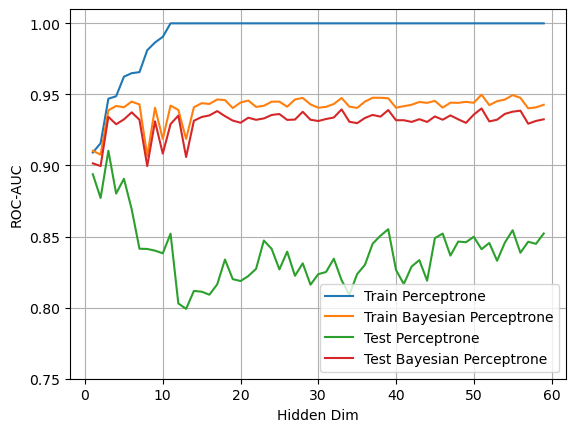
\includegraphics[width=1\linewidth]{roc_auc.png}
    \caption{Зависимость $ROC-AUC$ от размерности скрытого состояния на тренировочных и тестовых данных}
    \label{fig:enter-label}
\end{figure}

\section{Выводы}
По результатам работы можно сделать следующие выводы:
\begin{itemize}
    \item с ростом сложности модели байесовская нейронная сеть не переобучилась;
    \item значение ROC-AUC на тестовой выборке имеет очень высокую корреляцию со значением ROC-AUC на тренировочной выборке (0.97 по Пирсону). Следовательно, для подбора гиперпараметров можно ориентироваться на метрики, полученные по тренировочной выборке. Это даёт нам возможность отказаться от деления на тренировочную и валидационную выборки для подбора гиперпараметров.
\end{itemize}

Так же стоит отметить, что данный подход переносится на другие архитектуры нейронных сетей (рекуррентные, свёрточные, трансформеры).

Имплементация данного подхода была выполнена с использованием PyTorch. Весь исходный код для проведения экспериментов размещён по адресу \url{https://github.com/dimabasow/bayesian-neural-networks}.

\end{document}
